\section{多任务视角下的水印去除}
\label{sec:multitask}

\subsection{“盲”设置下的水印去除}

如前文所述,由于水印图案本身及其在嵌入过程中的复杂多变,没有用户指导或强约束的前提下难以很好地检测和去除它们。但是,在“盲”设定下,这些图案的确切位置、结构和大小是未知的。先前的方法依赖于恢复受损像素的位置信息,即使是深度学习的方法也都依赖于分阶段地对水印嵌入位置进行检测。Hert 等~\cite{hertz2019blind}首次提出了一种完全“盲”的视觉图案去除方法,该网络可以移除在训练过程中未见过的视觉图案,例如从真实世界图片中去除水印。网络首先估计哪些像素包含图案,然后重建潜在图像来分离视觉图案和图像。除了估计二值图案掩模和重建潜在图像之外,该网络还重建了嵌入到载体图像的视觉图案。将输入图像分解为视觉图案和背景图像(载体图像)使网络能够更好地重建图像。

\begin{figure}[!htbp]
	\centering
	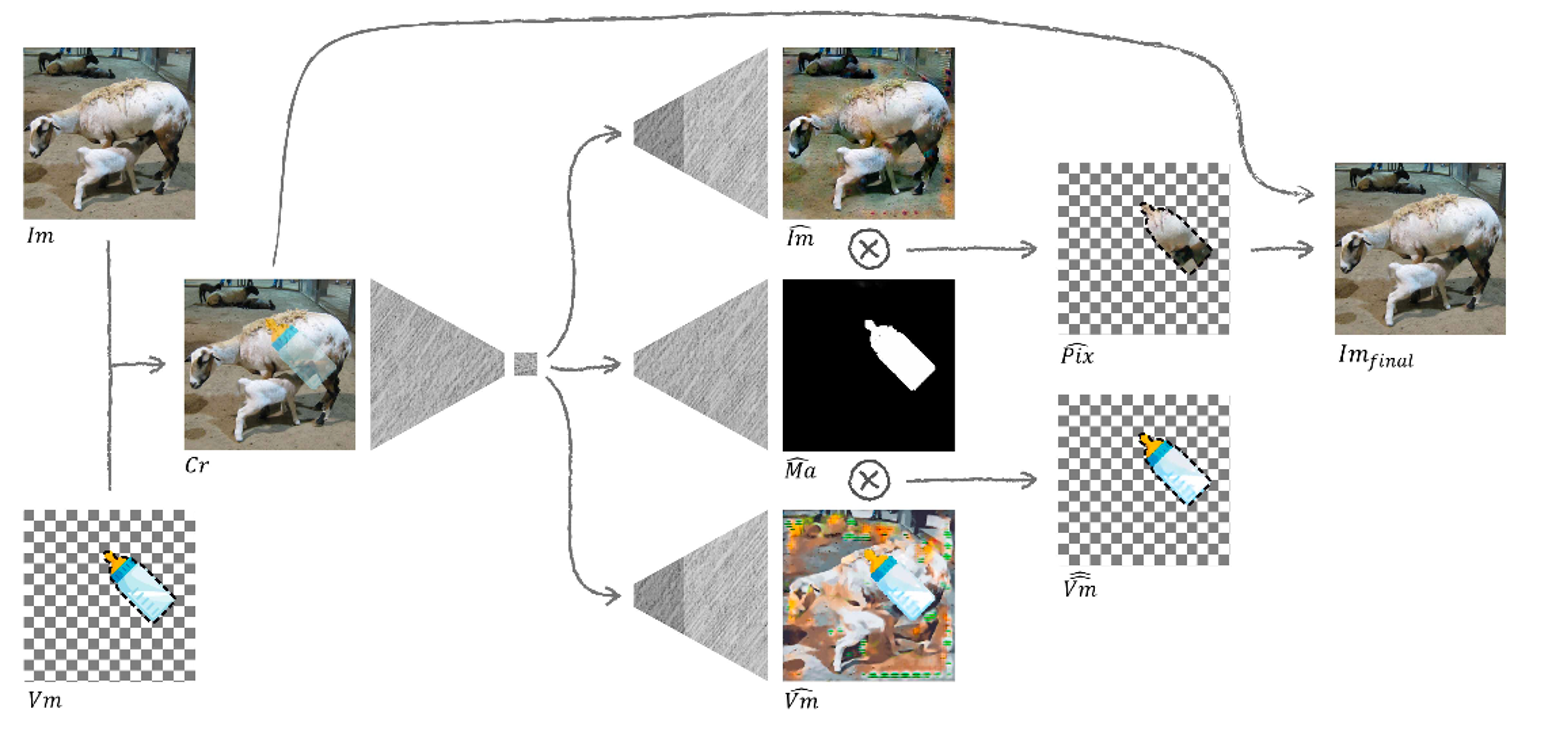
\includegraphics[width=\columnwidth]{27.png}
	\caption{“盲”设定下的多任务水印提取和图像恢复网络架构图}
	\label{fig:27}
\end{figure}

网络通过编码器将嵌入了水印的图像编码为潜在表示,然后通过三个并行的解码器分支进行解码:一个用于估计潜在图像,一个用于估计图案掩模,一个用于估计图案图像。最终的图像通过使用估计的图案掩模从输入图像或重建图像中选择像素来生成。在训练过程中,使用输入图像和视觉图案作为真值来计算损失以优化编码器和解码器网络。

\begin{figure}[!htbp]
	\centering
	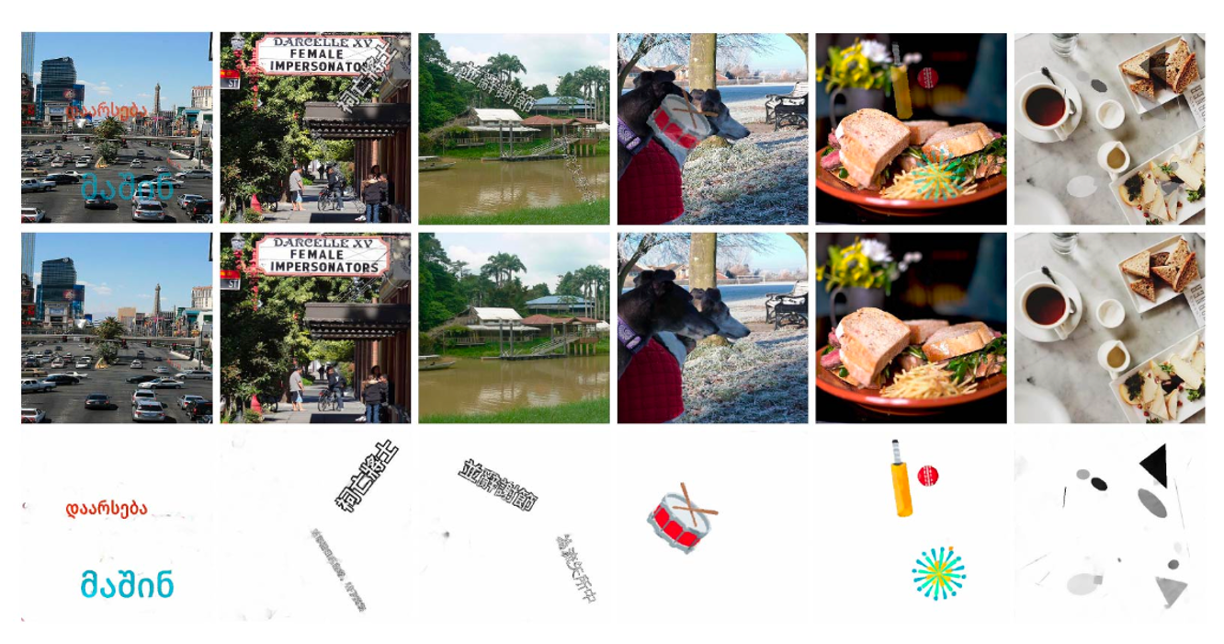
\includegraphics[width=\columnwidth]{28.png}
	\caption{水印提取和图像恢复结果}
	\label{fig:28}
\end{figure}

\subsection{显示建模水印区域的复原网络}

先前的研究将水印去除视为图像到图像的转换任务,并使用生成对抗网络将带有水印的图像直接映射到无水印图像。受益于GAN在图像转换方面的强大能力,这些方法取得了出色的去除性能。但是,这些方法与传统方法相比的一个不足之处是不能将水印与输入图像分离。将水印与输入图像分离使得更容易利用水印,从而有助于加强对去除攻击的抵抗能力。此外,通过将这些分离的水印应用于无水印图像来增加训练数据,可以使模型在不同水印上具有更好的泛化能力,进而提高推断性能。

\begin{figure}[!htbp]
	\centering
	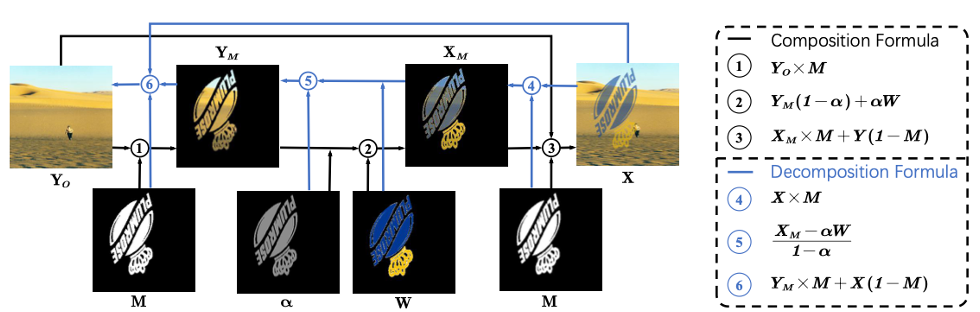
\includegraphics[width=\columnwidth]{29.png}
	\caption{水印嵌入过程和反过程示意图}
	\label{fig:29}
\end{figure}

受上述分析的驱动,Liu等~\cite{liu2021wdnet}拟在神经网络的生成器中构建水印图像的组合机制,其设计的WDNet具有深度学习方法从大规模数据集中学习的巨大能力,又兼具传统方法将水印与输入图像分离的能力。WDNet与先前的方法之间一个显著的区别是WDNet采用了两阶段的改进策略。Liu等认为水印去除任务隐含了一个预处理步骤——水印区域定位,这在先前的方法中被忽略了。因此,在WDNet的设计中显式地建模了这一过程,使得WDNet自然成为一个两阶段的生成器。

在第一阶段,WDNet不是直接估计无水印图像,而是通过预测粗糙的水印及其透明度来估计水印的大致区域,即($\hat{\alpha}, \hat{W}, \hat{M}$)。然后,根据网络估计的先验信息及水印嵌入的逆过程可以获得初步的无水印图像。然而,这一初步的结果并不令人满意,因为($\hat{\alpha}, \hat{W}, \hat{M}$)的值可能相互冲突,导致结果不够平滑。此外,这个结果仅粗略地表示了水印区域,需要进一步的细化。因此,在获得初始分解的无水印图像后,WDNet的第二阶段旨在通过从输出中获得额外的监督来对这些图像进行优化。由于第二阶段要求网络集中在像素级的细化上,而不是大范围和冗余的上下文,故此使用一个非常小的网络作为第二阶段的优化网络。具体来讲,它由几个残差块组成,有助于保证局部细化和高效性。和之前的工作类似,WDNet在第一阶段采用了U-Net的网络结构,并采用了基于补丁的鉴别器进行对抗训练。此外,WDNet不需要任何后处理过程。

\begin{figure}[!htbp]
	\centering
	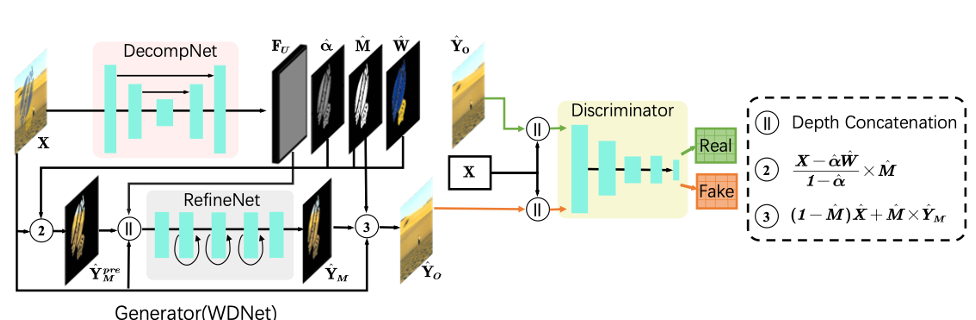
\includegraphics[width=\columnwidth]{30.png}
	\caption{WDNet架构图}
	\label{fig:30}
\end{figure}

\subsection{构建高效的水印去除模型}

在先前的工作中,检测水印位置是去除水印的前提,在获得水印嵌入位置后,可以通过图像修复或特征匹配来去除水印。Hertz等首次使用多任务网络来“盲”地从单幅图像中去除水印。然而,Liu等认为显示地学习水印嵌入区域是必要的。这种两阶段框架的基本思想是在多任务学习的架构下,由于嵌入水印图案与载体图像的纹理不协调,水印去除比检测更加复杂,因而需要对初步估计的原始图像进一步细化。如果背景(b)、预测掩码(e)和水印(g)由同一个网络生成,则背景(b)的视觉质量较差。其原因是因为水印去除需要从退化区域恢复确切的像素值,而水印检测只需要获取二进制掩码。因此,尽管可以像Hertz等那样使用单个多任务网络进行水印去除,但仍然需要使用预测的掩码(e)通过另一个网络对水印区域进行优化。基于上述分析,Cun等~\cite{cun2021split}提出了注意力引导的两阶段框架SplitNet和RefineNet。

\begin{figure}[!htbp]
	\centering
	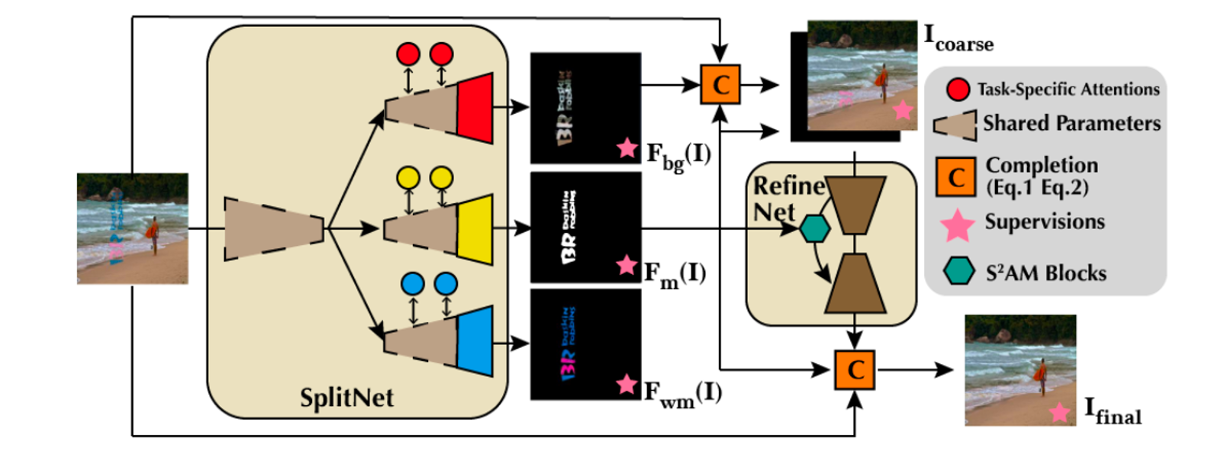
\includegraphics[width=\columnwidth]{31.png}
	\caption{两阶段网络架构图}
	\label{fig:31}
\end{figure}

在第一阶段,SplitNet使用基于残差块的U-Net作为基本的编码器-解码器结构,通过一个共享的编码器和多个解码器同时预测水印、背景和掩码,联合学习多个相关目标可以提升单个任务的性能。同时,将联合学习框架视为多域学习问题。在多域学习中,尽管每个域需要使用不同的参数,但为了学习一个高效的模型,几乎所有网络参数在训练过程中都是共享的。类似地,SplitNet中的三个任务在专注于学习一个空间区域的同时,每个任务都必须学习其重建任务相关的特定特征。具体而言,SplitNet三个解码器共享参数,并通过单独的域注意力学习每个任务的特定特征。这种策略有助于构建更高效和有效的模型。

在第二阶段,RefineNet,使用预测的掩码和SplitNet中的粗略结果进一步细化掩码区域像素。如果直接将掩码和粗糙结果作为第二阶段的输入,那么简单的网络可能无法专注于学习水印区域。因此,受空间分离注意力模块(S2AM)在图像和谐化中应用的启发,通过引入基于注意力的网络来改进预测的掩码区域。

\subsection{高质量掩膜预测的水印去除网络}

现有的水印去除方法可以分为两大类:(1) 端到端的全图擦除;(2) 同时检测水印和修复背景。第一种方法将水印去除的任务视为一个图像翻译的任务,即将带有水印的图片作为源域,无水印的图片作为目标域,通过近些年流行的图像翻译模型,实现水印擦除的功能,然而这样的方法只是隐式地告知模型水印的区域,很容易使得模型误擦除物体。第二种方法则是一种多任务的学习框架,同时执行水印检测与图像修复的任务,这样一来,在最后的图片修复中,模型只需要修复检测出来的水印区域,大大减小了误擦除的可能性。

对于前者而言,水印掩膜对于最终的图像修复质量非常重要,然而现有方法都没有针对水印检测做出优化。在实际应用中,水印的主体图案很容易被模型检测出来,然而水印周边的附属文字或者图案却很容易被模型视为噪声而忽视,这样检测出来的水印质量较差,而且会降低后续的修复的图像质量。

\begin{figure}[!htbp]
	\centering
	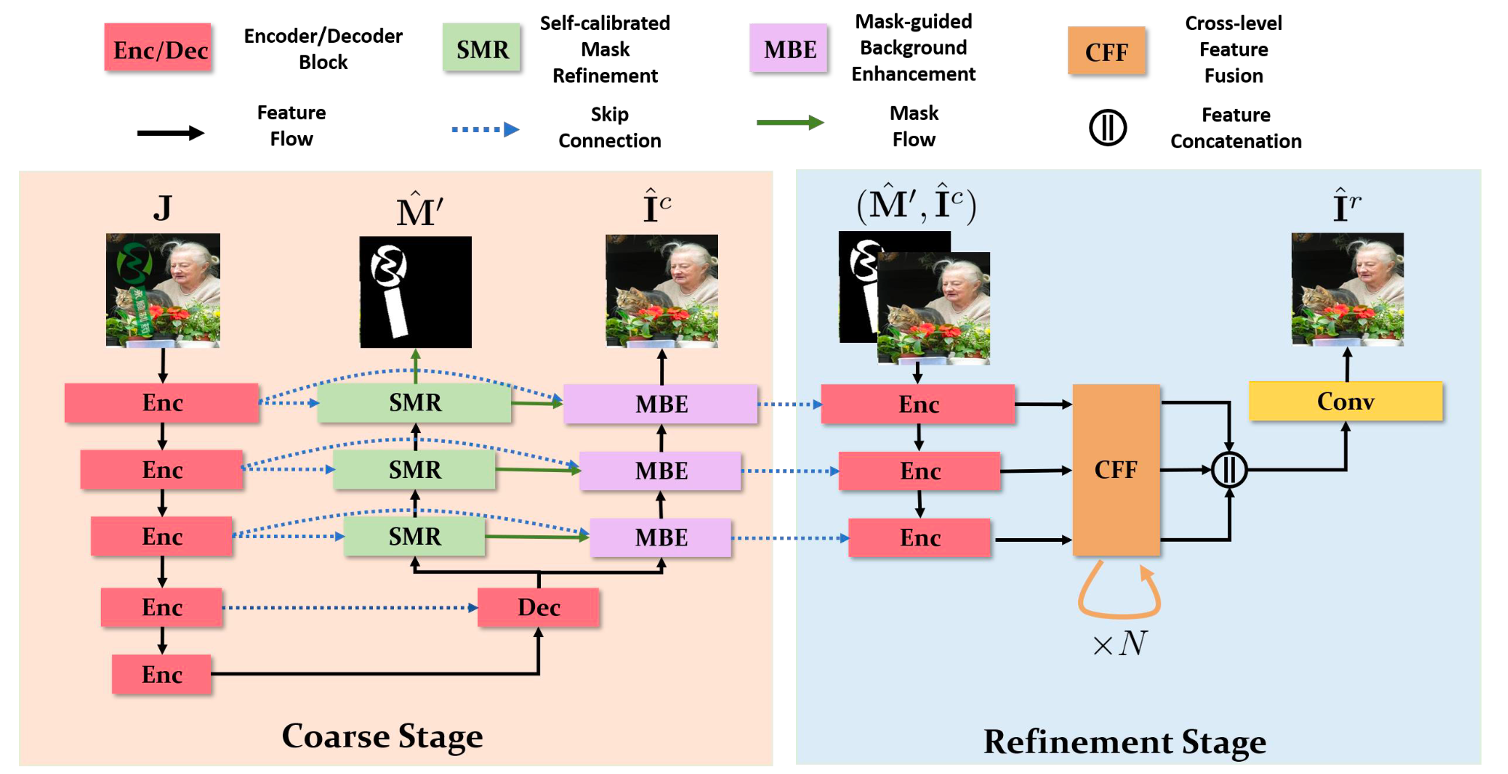
\includegraphics[width=\columnwidth]{32.png}
	\caption{基于自纠正水印检测模块和掩膜指引背景修复模块的可见水印去除网络架构图}
	\label{fig:32}
\end{figure}


为此,Liang等~\cite{liang2021visible}提出了自纠正的水印检测模块(Self-calibrated Mask Refinement),掩膜指引的背景修复模块,多层次信息融合的背景改进模块。整体框架可以分为背景粗修阶段,以及背景精修阶段。在背景粗修阶段,将水印定位和水印去除作为多任务学习框架中的两个任务。具体来说,网络由传统的U-Net结构演变而来,为了兼顾模型大小以及多任务的需求,采用了共享编码器以及一层共享解码器的主干网络,对于水印掩膜检测以及背景修复任务,则采用了不同的解码器分支实现不同的功能。掩膜解码器分支预测多尺度水印掩膜,通过掩膜引导的背景增强(MBE)模块为背景解码器分支提供指导,以更好地重建无水印图像。考虑到不同图像中的水印在许多方面存在很大的差异,设计了一个自校准掩膜细化(SMR)模块,将水印特征传播到整个特征图中,以更好地处理特定于图像的水印。在背景精修阶段,以预测的水印掩膜和粗度阶段的无水印图像作为输入,生成一个细化的无水印图像。为了充分利用粗修阶段的有用信息,在粗修阶段的背景解码器分支和细化阶段的编码器之间添加了跳连接。考虑到不同层次的特征捕获了结构信息或纹理细节,在精修阶段反复使用跨层次特征融合(CFF)模块来聚合多层次编码器特征。从精修阶段得到的输出图像是最终恢复的背景图像。

\begin{figure}[!htbp]
	\centering
	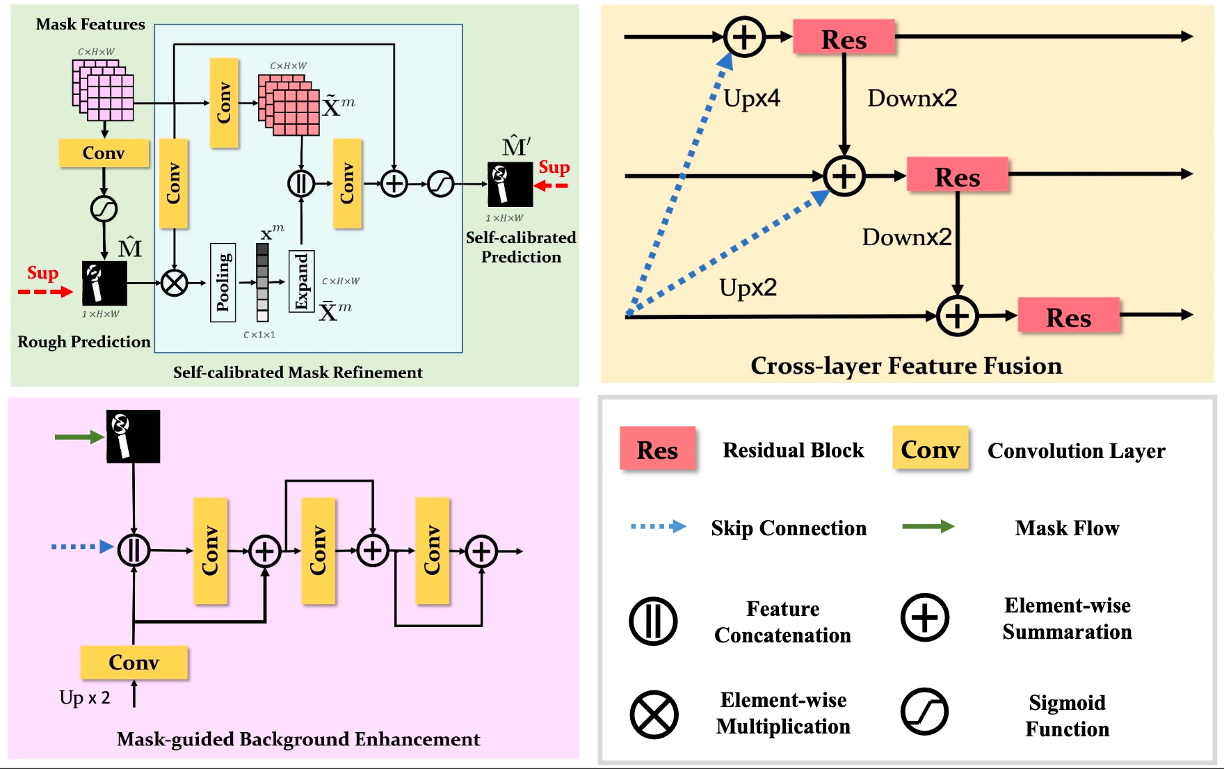
\includegraphics[width=\columnwidth]{33.png}
	\caption{自纠正的水印检测模块,掩膜指引的背景修复模块和多层次信息融合的背景改进模块示意图}
	\label{fig:33}
\end{figure}


自纠正水印检测模块分为两个部分,一个是常规的水印检测部分($X^m$以及$\hat{M}$),另一部分则是纠正掩膜的部分。在自纠正部分,作者希望学习到水印主图案的特征,将其在隐空间的特征与水印掩膜其他位置特征做相似度匹配,以此找出可能的环绕图案。在纠正模块中,首先从预测得到的水印掩膜的置信度图中,取出高置信度的掩膜,这一区域可以被认为代表了水印主体图案,随后将高置信度的掩膜与掩膜特征做点乘,并求平均得到一个均值向量$x^m$, 该向量可以表示为水印掩膜的主要特征;然而环绕在主图案的水印外表特征可能与主图案不一致,因此将水印掩膜主特征$x^m$投影到一个隐空间,得到$\bar{X}^m$,同时将水印特征也投影到隐空间,得到$\tilde{X}^m$,在此隐空间里将两个投影特征级联,通过1x1的卷积,即一个变换矩阵,学习相似度,最后得到了一个相似度图,在此相似度图里,只考虑正相关部分,因此可以使用水印掩膜标注作为监督,如此,可以识别出一些漏检并消除一些误报。

水印掩膜指引修复模块引入了预测的掩膜图作为指导。在跨层次特征融合中,考虑到分辨率较小的深层特征能够融合更多的语义信息,因此将其作为自下而上传播的特征流,在此结构中,可以看到信息可以自上而下以及自下而上的流动,充分地融合了背景修复的信息。

\begin{figure}[!htbp]
	\centering
	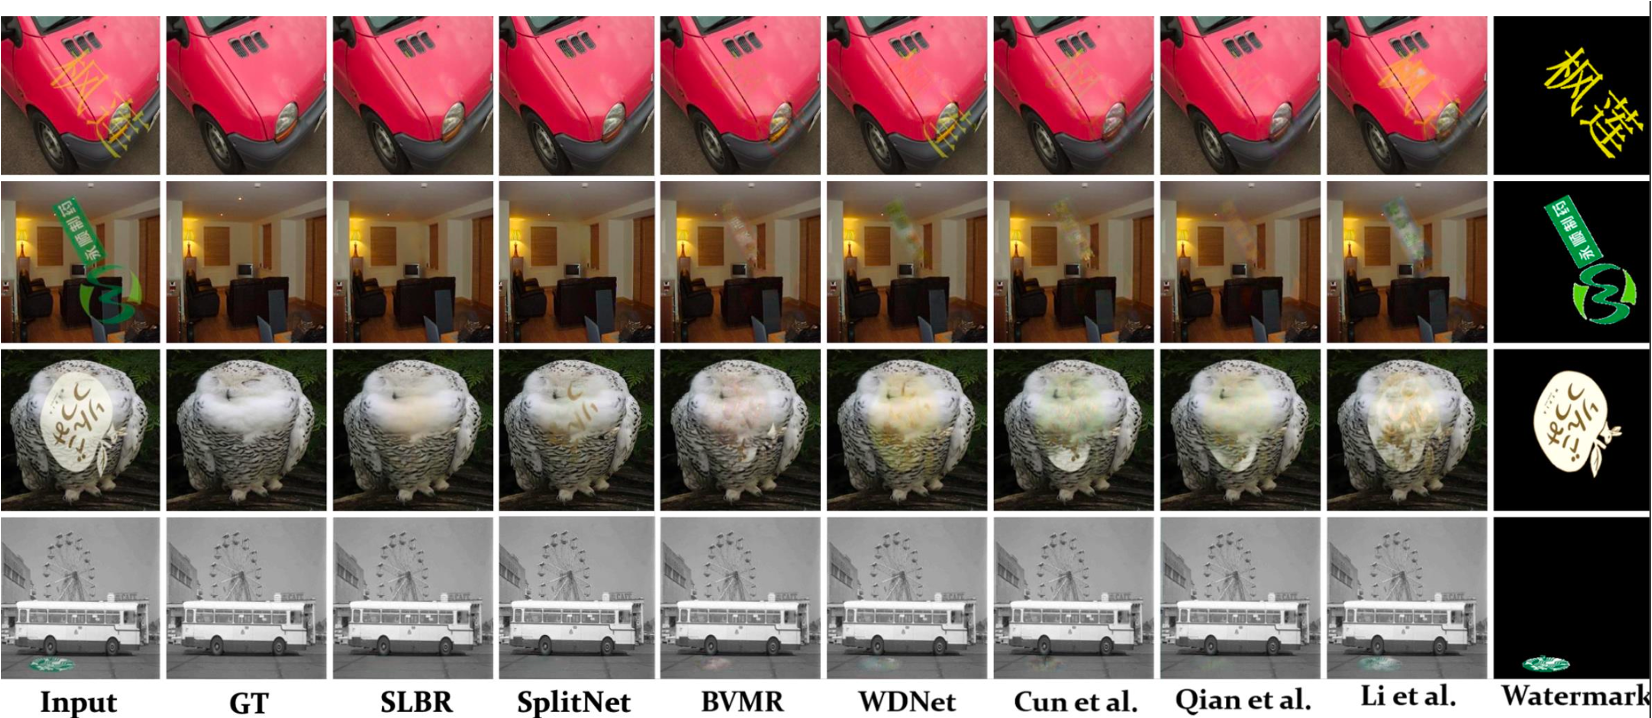
\includegraphics[width=\columnwidth]{34.png}
	\caption{水印去除结果示例图}
	\label{fig:34}
\end{figure}